\section{Introduction}
Started back in 1952, when IBM first manufactured large computer system and sold into the market as mainframe. It was bulky, large, and expensive machine that take up a room size. More importantly, every components within that mainframe is IBM's proprietary hardware, which means, a customer have to buy the whole vertically integrated solution from a single vendor regardless of the solution they want to have for their problem (software calculation, hardware design, finance...).
\begin{figure}[H]
    \centering
    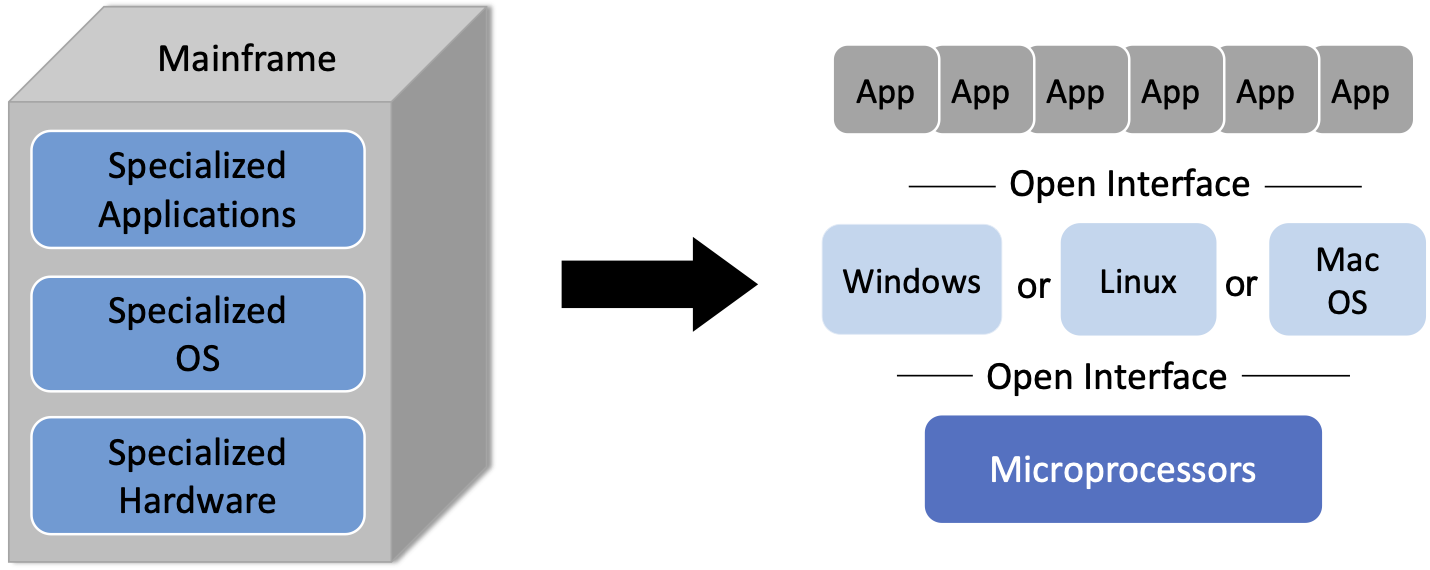
\includegraphics[width=1\linewidth]{graphics/vertical integrated solution.png}
    \caption{Transformation from vertical market to horizontal marketplace with open interfaces at all level. Adapted from \cite{systemsapproach}.}
    \label{fig:vertical-integration}
\end{figure}
The evolution began with the arrival of open-source operating systems and microprocessors, which helped transform the market into a horizontal one where innovation could happen at any layer.

SDN initiatives draw the similar inspiration by decoupling the control plane from the data plane. Decision-making logic is decided by a external\footnote{In SDN terminology, a distinction exists between \textbf{external (global) network OS} and the \textbf{internal (local) network OS}. The External NOS referrs to a distributed controller platform to maintain a centralized view of the network (ONOS section) while Internal OS refers to lightweight OS running directly on-switch to manage internal switch operation and communicate with the external network OS.} logically centralized controller\footnote{While SDN control plane is logically centralized to provide a unified global view of network state and simplify network management, production deployment (introduced in ONOS section) are physically distributed for high availability and scalability}, using information from network operating systems enabled on top of the underlying switches. This abstraction simplifies switch's role, off-loading complex decision making logic (i.e., routing, path computation, ACL..) off-device and reducing the switch's primary task to packet forwarding. So they are referred to as "white box" or "bare-metal" switches\footnote{"bare-metal" switches run a ONIE bootloader uses facilities in Linux kernel and BusyBox, defining an open source "install environment" for end users to install target network OS~\cite{onie}} which doesn't come with a fixed network OS, creating a hardware ecosystem for multiple operating system vendors.

OpenFlow is the pioneer protocol that support this disaggregation in the early stage of SDN. Although it was a main instrumental propelling SDN into the mainstream, OpenFlow now play a small role of today SDN because of an architectural limitation it imposed---namely, its fixed-function match-action pipeline. Modern infrastructure has largely transitioned toward fully programmable data planes driven by the P4 programming language, P4Runtime, and Stratum. The objective of this study is to explore this architectural evolution from early OpenFlow to current P4-based ecosystems deployed across large-scale hyperscale data centers. Unless otherwise noted, the architectural exposition in the remainder of this report, including the accompanying figures, follows the treatment given in \cite{systemsapproach}.
